% =====================================================================
%  CHAPTER 3: METHODOLOGY
%  Safe helper macros (\providecommand never overrides an existing macro)
% =====================================================================
\providecommand{\mpnet}{\texttt{paraphrase-\allowbreak multilingual-\allowbreak mpnet-\allowbreak base-\allowbreak v2}}
\providecommand{\cemodel}{\texttt{ms-marco-\allowbreak MiniLM-\allowbreak L-6-\allowbreak v2}}
\emergencystretch=3em
\providecommand{\pending}[1]{\textbf{[PENDING: #1]}}

\chapter{Methodology}
\label{chap:methodology}

This chapter describes how the explainable reviewed-item retrieval system was designed, built, and evaluated. The study is organised around three research questions that were refined after the feedback received on the project proposal. The first asks whether lexical (BM25) and dense retrieval remain competitive when both score the same retrieval unit and when sentence-level scores are aggregated into a restaurant score, and whether those aggregations are biased by the number of reviews a restaurant has. The second asks whether the review sentences shown to the user as an explanation genuinely support the restaurant ranking. The third asks whether the sentence-retrieval step transfers to real Thai restaurant reviews that are judged against independently annotated taste preferences.

The chapter is divided into six sections. Section~\ref{sec:datasets} introduces the datasets that were used in the final study, and Section~\ref{sec:eda} reports the exploratory data analysis (EDA) together with the design decisions that followed from it. Section~\ref{sec:preprocessing} documents data preprocessing and feature preparation. Section~\ref{sec:models} defines the baseline model, the proposed model, the aggregation functions, and the retrieval extensions that were tested. Section~\ref{sec:pipeline} presents the end-to-end pipeline and its implementation, and Section~\ref{sec:evalprotocol} describes the evaluation protocol used for the English ranking experiments, the explanation experiments, and the Thai case study.

% ---------------------------------------------------------------------
\section{Datasets Used}
\label{sec:datasets}

Two datasets carry the quantitative and qualitative evaluation in the final study. They play complementary roles, because no single public dataset provides restaurant-level grouping, free-text preference queries, human relevance labels, and Thai text at the same time.

\subsection{RIRD: Reviewed-Item Retrieval Dataset}
\label{sec:rird}

The Reviewed-Item Retrieval Dataset (RIRD) was released with the reviewed-item retrieval task of \citet{abdollahpour2023} and is the only source of independent human relevance judgements used in this project. It consists of two linked files. The review file contains 29,168 English reviews of 50 Toronto restaurants, with the restaurant identifier, reviewer identifier, star rating, review text, restaurant name, cuisine categories, and review date for each review. The second file, \texttt{PMD.csv}, contains 100 free-text preference queries, each judged against all 50 restaurants. This yields 5,000 query--restaurant pairs after one exact duplicate row is removed, and every pair carries binary relevance judgements from five annotators together with an aggregated binary label. The aggregated label is the ground truth used for every ranking metric reported in Chapter~\ref{chap:results}.

\subsection{Wongnai Reviews}
\label{sec:wongnai}

The Wongnai review corpus \citep{highgroundbkk} contains 40,000 training and 6,203 test restaurant reviews written in Thai. Each record has only two fields: the review text and a customer satisfaction rating on a 0--4 scale. The corpus has no restaurant identifier, no query field, and no relevance label of any kind. It therefore cannot support restaurant-level ranking evaluation, which is the reason why it is used only for a sentence-level Thai case study in which we supply our own taste queries and our own human relevance labels (Section~\ref{sec:thaieval}).

\subsection{Datasets Excluded from the Final Study}
\label{sec:excluded}

The project proposal also listed the Thailand Foods dish gazetteer and the Thai subset of M-ABSA as supporting resources for an optional flavour-feature layer. After the proposal feedback, the scope was narrowed to questions that could be measured with the available labels, and both datasets, together with Thai restaurant-level ranking, were declared out of scope. They were explored during the proposal phase but contribute no result in this report.

% ---------------------------------------------------------------------
\section{Exploratory Data Analysis}
\label{sec:eda}

Exploratory analysis was carried out separately for the two datasets because they serve different purposes. RIRD is the measured evaluation set, so its analysis focuses on the properties that influence evaluation design, such as review volume per restaurant, label imbalance, and annotator agreement. Wongnai is inspected to establish exactly what kind of experiment it can support.

\subsection{RIRD Reviews}
\label{sec:edarird}

The review file contains 29,168 reviews written by 17,334 distinct users about 50 restaurants, with review dates between 2008 and 2019. No missing values were found in the fields used downstream and there are no duplicate rows. The distribution of review counts across restaurants is highly unequal: individual restaurants have between 406 and 2,281 reviews. This imbalance matters because aggregation functions such as the maximum or a top-$k$ mean can favour restaurants with more review text simply because more sentences give more chances of a high score. It motivated the explicit volume-control experiment described in Section~\ref{sec:volumecontrol}.

Star ratings skew strongly towards the positive end (Figure~\ref{fig:rirdstars}), with a mean rating of 3.93, which is consistent with the source dataset's restriction to restaurants with an average rating of at least three. Review length is right-skewed with a long tail and a median of approximately 94 words (Figure~\ref{fig:rirdlength}). A long review contains many different statements about food, service, price, and atmosphere, so a single review-level vector or score blends signals that a query may only care about in one sentence. This observation supports splitting reviews into sentences before encoding.

\begin{figure}[htbp]
    \centering
    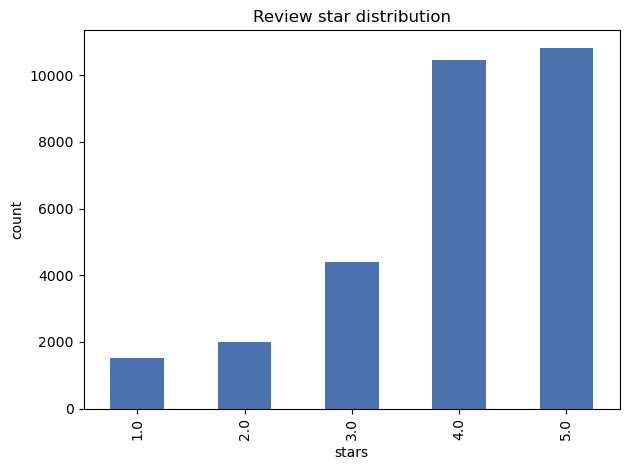
\includegraphics[width=0.8\textwidth]{figures/rird_star_distribution.png}
    \caption{Distribution of review star ratings in RIRD.}
    \label{fig:rirdstars}
\end{figure}

\begin{figure}[htbp]
    \centering
    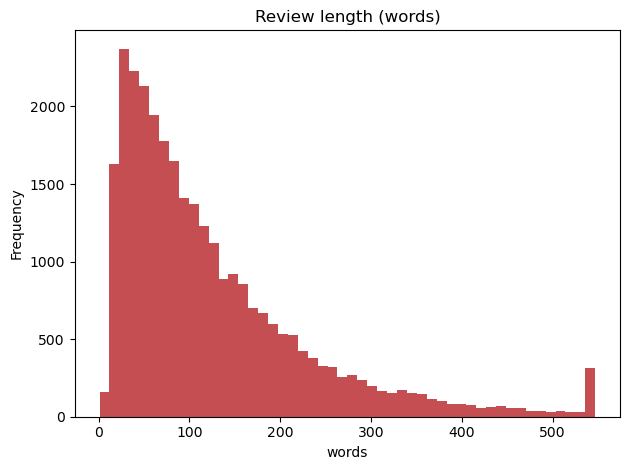
\includegraphics[width=0.8\textwidth]{figures/rird_review_length.png}
    \caption{Distribution of RIRD review length in words (clipped at the 99th percentile).}
    \label{fig:rirdlength}
\end{figure}

\subsection{RIRD Relevance Labels}
\label{sec:edapmd}

After removing one exact duplicate row, the PMD file contains 5,000 query--restaurant judgements (100 queries $\times$ 50 restaurants). The aggregated label is positive for approximately 27\% of the pairs, which corresponds to an average of 13.5 relevant restaurants per query out of 50. Figure~\ref{fig:pmdvotes} shows how many of the five annotators voted a pair relevant; the mass at zero votes confirms that the positive class is a clear minority. Inter-annotator agreement reported with the RIRD release is Cohen's $\kappa \approx 0.528$ \citep{abdollahpour2023}, which indicates moderate agreement and reminds us that relevance for subjective preference queries is partly a matter of opinion.

Because only about one pair in four is positive, accuracy-style metrics would be misleading: a system that labels every restaurant as irrelevant would already be right about 73\% of the time. For this reason all English experiments use rank-aware metrics (nDCG, MAP, MRR, precision, and recall at a cut-off), as described in Section~\ref{sec:englisheval}. The PMD file has no query-category column, so a per-category breakdown (for example indirect, negation, and contradictory queries) was not possible.

\begin{figure}[htbp]
    \centering
    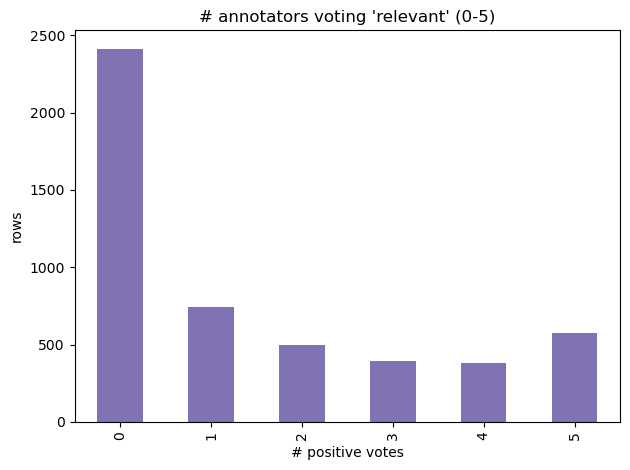
\includegraphics[width=0.8\textwidth]{figures/pmd_annotator_votes.png}
    \caption{Number of annotators (out of five) voting a query--restaurant pair relevant.}
    \label{fig:pmdvotes}
\end{figure}

\subsection{Wongnai Reviews}
\label{sec:edawongnai}

The Wongnai ratings are concentrated at the middle of the 0--4 scale (Figure~\ref{fig:wongnaistars}), and review text is much shorter than in RIRD, with a median of approximately 20 whitespace-delimited tokens (Figure~\ref{fig:wongnailength}). A language screen shows that roughly 99\% of the text is Thai, either purely Thai or mixed with some English. The most important finding is structural rather than statistical: the corpus contains no restaurant identifier, query, or relevance label. This single fact rules out restaurant-level evaluation on Wongnai and determines the design of the Thai track.

\begin{figure}[htbp]
    \centering
    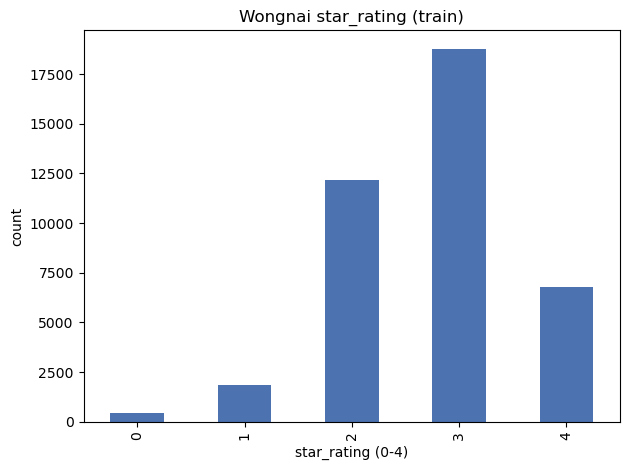
\includegraphics[width=0.8\textwidth]{figures/wongnai_star_distribution.png}
    \caption{Distribution of Wongnai star ratings (0--4 scale).}
    \label{fig:wongnaistars}
\end{figure}

\begin{figure}[htbp]
    \centering
    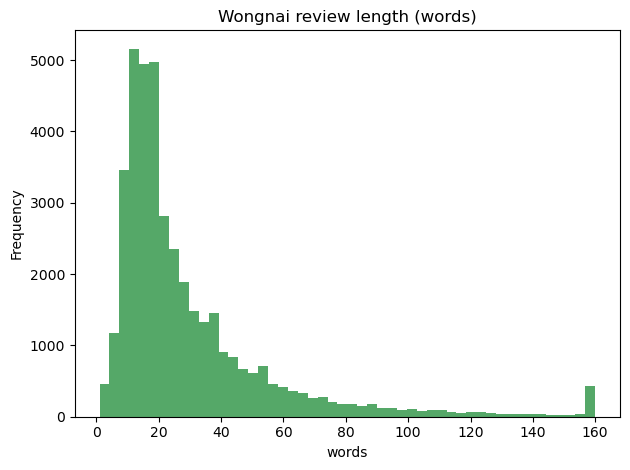
\includegraphics[width=0.8\textwidth]{figures/wongnai_review_length.png}
    \caption{Distribution of Wongnai review length in words (clipped at the 99th percentile).}
    \label{fig:wongnailength}
\end{figure}

\subsection{Language Composition Check}
\label{sec:langcheck}

A Unicode-range script detector was applied to a random sample of 5,000 reviews from each corpus. In RIRD, 100\% of the sampled review text and all 100 PMD queries are Latin-script English, and no Thai content is present. In Wongnai, the sample is overwhelmingly Thai script. These results lead to a strict rule that was followed throughout the project: Thai queries are never run against RIRD, because there is nothing Thai to match, and English evaluation claims are never made on Wongnai.

\subsection{Summary of EDA Findings and Design Decisions}
\label{sec:edasummary}

Table~\ref{tab:edadecisions} summarises how each EDA finding translated into a concrete design decision. Every major choice in the preprocessing and evaluation design is traceable to an observed property of the data.

\begin{table}[htbp]
\centering
\caption{EDA Findings and the Design Decisions They Motivated}
\label{tab:edadecisions}
\small
\begin{tabular}{|p{0.38\textwidth}|p{0.54\textwidth}|}
\hline
\textbf{EDA finding} & \textbf{Design decision} \\
\hline
RIRD reviews are long and right-skewed (median about 94 words) & Split reviews into sentences and retrieve at sentence level \\
\hline
Reviews per restaurant range from 406 to 2,281 & Run a review-volume control and include a review-count baseline \\
\hline
About 27\% of PMD pairs are relevant & Use rank-aware metrics instead of accuracy \\
\hline
RIRD text and queries are 100\% English & Measure restaurant ranking in English only \\
\hline
Wongnai has no restaurant id, query, or label & Run a sentence-level Thai case study with our own queries and human labels \\
\hline
Thai is written without spaces between words & Use PyThaiNLP for sentence segmentation and word tokenisation \\
\hline
\end{tabular}
\end{table}

% ---------------------------------------------------------------------
\section{Data Preprocessing}
\label{sec:preprocessing}

\subsection{Missing Values and Duplicates}
\label{sec:missing}

Missing values in the RIRD cuisine category field are filled with the label ``Unknown'', and the review text, rating, and restaurant identifier used downstream contain no missing values. The single exact duplicate row in \texttt{PMD.csv} was dropped before evaluation, leaving 5,000 judgements. In Wongnai, the review text is the primary field and is never null, so no imputation was necessary. The Wongnai star rating is not used as a regression target or filter in the final experiments, and the non-standard 0--4 scale therefore required no transformation.

\subsection{Outliers and Very Short Texts}
\label{sec:outliers}

Reviews shorter than ten words were flagged as possible near-empty entries and were retained unless they were entirely blank, because a short review can still contain a valid preference statement. The positive rate of about 27\% in PMD is not treated as an outlier; it is an expected consequence of how sparse relevance is for preference queries, and it informed the choice of metrics. A related issue appeared later at sentence level: very short sentences such as ``Solid meal!'' can receive deceptively high similarity scores with short queries. In the 375 evidence sentences sampled for human support rating, 169 (45.1\%) contained fewer than ten whitespace-delimited words. This finding motivated a minimum-length filter in the live system (Section~\ref{sec:livefilter}).

\subsection{Distribution and Skewness}
\label{sec:skew}

Review lengths in both corpora are right-skewed. Rather than transforming or clipping the data, the skew is handled structurally: every review is split into sentences before encoding, so that the unit of retrieval is the sentence and a small number of very long reviews cannot dominate a restaurant's score through sheer length. The ratings in Wongnai are concentrated in the middle of the scale, but since ratings do not enter the retrieval pipeline, this has no effect on the results.

\subsection{Sentence Segmentation and Tokenisation}
\label{sec:segmentation}

English reviews were split into sentences with the NLTK sentence tokenizer, which produced a corpus of 240,660 retrieval units for the 29,168 RIRD reviews. Thai reviews were split into sentences with the \texttt{crfcut} segmenter of PyThaiNLP\footnote{\url{https://github.com/PyThaiNLP/pythainlp}}, because Thai is written without spaces between words and without reliable sentence-final punctuation. A random sample of 10,000 Wongnai reviews (random seed 42) produced 93,810 sentences, an average of 9.4 sentences per review. A segmentation spot-check on a 2,000-review development subsample was performed by a Thai-speaking team member before the larger run. For the BM25 baseline, English text was lower-cased and stripped of punctuation, and Thai text was tokenised with the \texttt{newmm} dictionary-based tokenizer of PyThaiNLP.

\subsection{Feature Preparation}
\label{sec:features}

All queries and retrieval units are encoded into a shared vector space with the pretrained multilingual sentence-transformer \mpnet{}, which produces 768-dimensional embeddings \citep{reimers2019}. The encoder is used frozen and off the shelf, with no fine-tuning, and sentence embeddings are computed once and cached. For the RIRD sentence corpus, the cache is a matrix of 240,660 $\times$ 768 values of approximately 740 MB. Relevance is computed with cosine similarity, which is invariant to vector length, so no additional feature scaling or normalisation step is applied. A maximum sequence length of 256 tokens is used when encoding sentences.

% ---------------------------------------------------------------------
\section{Models}
\label{sec:models}

\subsection{Problem Formulation}
\label{sec:formulation}

Let $R=\{r_1,\dots,r_n\}$ be the set of restaurants, where each restaurant $r_i$ has a set of reviews that is decomposed into a set of sentences $S_i=\{s_{i,1},s_{i,2},\dots\}$. Given a free-text query $q$, the system scores every sentence against the query, aggregates the sentence scores of each restaurant into a single restaurant score with a fusion function $f$, and ranks the restaurants by that score:
\begin{equation}
\mathrm{Score}(q,r_i) = f\big(\{\,\mathrm{score}(q,s_{i,j}) : s_{i,j}\in S_i\,\}\big).
\label{eq:fusion}
\end{equation}
The highest-scoring sentences of each restaurant are returned with the ranking as the explanation. For dense retrieval, the sentence score is the cosine similarity of the query embedding $\mathbf{e}_q$ and the sentence embedding $\mathbf{e}_s$:
\begin{equation}
\mathrm{score}(q,s)=\frac{\mathbf{e}_q\cdot\mathbf{e}_s}{\lVert\mathbf{e}_q\rVert\,\lVert\mathbf{e}_s\rVert}.
\label{eq:cosine}
\end{equation}

\subsection{Baseline Model}
\label{sec:baseline}

The baseline follows the standard lexical approach of the original reviewed-item retrieval work \citep{abdollahpour2023}. All reviews of a restaurant are concatenated into a single document, the 50 documents are indexed with the Okapi BM25 ranking function \citep{robertson2009} (implemented by the \texttt{rank-bm25} library), and each PMD query ranks the restaurants by their BM25 score. We refer to this model as \emph{BM25 on concatenated documents}. This was the first baseline implemented during the proposal phase, and it is the reference against which the proposed model is compared. A second proposal-phase baseline, \emph{dense pooled vector}, mean-pools the embeddings of all reviews of a restaurant into one 768-dimensional vector and ranks restaurants by cosine similarity to the query; it isolates the effect of using dense embeddings without any sentence-level fusion.

\subsection{Fair Comparison Design}
\label{sec:faircomparison}

The proposal feedback pointed out that the first baselines were not directly comparable, because BM25 scored one concatenated document per restaurant while the dense model scored mean-pooled reviews, and because fusion by maximum or top-$k$ might favour restaurants with many reviews. The final study therefore re-implements both retrieval models so that they score exactly the same retrieval unit and are aggregated with exactly the same set of functions. This was done at two granularities: \emph{review level}, where each review is one unit, and \emph{sentence level}, where each sentence is one unit. BM25 and dense retrieval are each paired with every aggregation function of Section~\ref{sec:aggregation}.

\subsubsection{Review-Volume Control}
\label{sec:volumecontrol}

To test whether the aggregation results are driven by the number of reviews, every restaurant was randomly subsampled to 400 reviews (random seed 42), which is possible because the smallest restaurant has 406 reviews. The correlation between a restaurant's score and its original review count was then compared before and after the control, and the ranking metrics were recomputed on the subsampled data.

\subsubsection{Query-Independent Floors}
\label{sec:floors}

Three query-independent rankings were included to show how much of the performance can be explained without reading the query: a random ranking (expected value), a ranking by the number of reviews of the restaurant, and a leave-one-out popularity ranking. The leave-one-out popularity score of restaurant~$r$ for query~$q$ is the number of queries \emph{other than} $q$ for which $r$ is relevant, so the ranking is query-conditioned without using $q$'s own labels.
\ These floors are useful because high scores for a model are only meaningful relative to what is achieved when the query is ignored.

\subsection{Aggregation Functions}
\label{sec:aggregation}

Let $x_{i,j}=\mathrm{score}(q,s_{i,j})$ denote the score of unit $j$ of restaurant $i$ for a given query, and let $\mathrm{top}_k(i)$ be the indices of the $k$ highest scores of restaurant $i$. The following fusion functions $f$ were compared, each applied identically to BM25 and dense scores:
\begin{align}
f_{\max}(i) &= \max_{j} x_{i,j}, \\
f_{\text{mean}}(i) &= \frac{1}{|S_i|}\sum_{j} x_{i,j}, \\
f_{\text{top-}k}(i) &= \frac{1}{k}\sum_{j\in \mathrm{top}_k(i)} x_{i,j}, \qquad k\in\{3,5,10\}.
\end{align}
Maximum pooling rewards a single strong sentence but is sensitive to noise and to the number of units. The mean over all units rewards consistent evidence but is diluted by irrelevant sentences. The top-$k$ mean sits between the two by averaging only the best $k$ units, which gives a more stable estimate than the maximum while ignoring the many sentences of a review that do not concern the query. The rating-weighted fusion listed in the proposal was not carried into the final study, in line with the revised scope.

\subsection{Proposed Model}
\label{sec:proposed}

The proposed model is \emph{sentence-level dense retrieval with top-10 mean aggregation}. Each review is split into sentences, the query and every sentence are encoded with \mpnet{}, every sentence is scored by cosine similarity (Equation~\ref{eq:cosine}), and the score of a restaurant is the mean of its ten highest sentence scores (Equation~\ref{eq:fusion} with $f_{\text{top-}10}$). Restaurants are ranked by this score and the top-scoring sentences of each restaurant are attached as explanation. This configuration was chosen as the proposed model because it achieved the best nDCG@10 and MAP among the fusion variants (Chapter~\ref{chap:results}). The model requires no training: the encoder is frozen and the only free choices are the aggregation function and the value of $k$.

\subsection{Retrieval Extension: Query Rewriting and Cross-Encoder Re-ranking}
\label{sec:b3}

Inspection of the human support labels (Section~\ref{sec:b2design}) revealed two systematic failure modes of the bi-encoder. The first is \emph{negation blindness}: because the encoder maps text to a point in a semantic space, a query such as ``no waitline'' and a sentence about a long wait are close to each other, as they discuss the same topic. The second is \emph{idiomatic query failure}: phrases such as ``cheat meal'' or ``I feel chubby'' have no direct food vocabulary and land in poorly defined regions of the embedding space. Two additions were implemented to address these problems and were evaluated as a single combined extension.

\paragraph{LLM query rewriting.} Before encoding, each query is rewritten by a large language model served through the Groq API (model \texttt{qwen/qwen3.8-27b}) into explicit, positively phrased keywords of the kind reviewers actually write. For example, ``no waitline'' is rewritten as ``quick seating walk-in no queue no reservation'', and ``cheat meal'' as ``indulgent rich comfort food burgers fries pizza calorie dense''. The rewritten query replaces the original query for the encoding step. The rewrites of all 100 PMD queries were cached so that the evaluation is repeatable.

\paragraph{Cross-encoder re-ranking.} A cross-encoder (\cemodel{}) reads the rewritten query and a candidate sentence jointly, with full attention between the two texts, and can therefore detect a mismatch that independent encodings cannot. Because a cross-encoder cannot use pre-computed embeddings, it is applied only to a restricted candidate set: the top 20 restaurants of the bi-encoder ranking and the 15 best bi-encoder sentences of each of them, which amounts to 300 cross-encoder evaluations per query instead of 1,500 in a naive implementation. The cross-encoder scores are then used to re-rank the restaurants.

\paragraph{Selective use.} The combined extension improved some queries and degraded others (Section~\ref{sec:resb3}). The live system therefore activates the cross-encoder only when the query contains an explicit negation or exclusion pattern, such as ``no'', ``not'', ``without'', ``don't'', ``never'', ``except'', ``avoid'', ``non-'', or ``instead of''. All other queries use the bi-encoder ranking directly.

\subsection{Choice of Models}
\label{sec:whymodels}

All models were chosen under a deliberate constraint of low complexity. No model is trained or fine-tuned: BM25 requires no learning, the sentence encoder is used frozen, and the aggregation functions have no learnable parameters. This makes every comparison attributable to a single design choice, namely the retrieval model, the retrieval unit, or the aggregation function, and it allows the whole study to run on a single consumer-grade GPU. The multilingual encoder was selected because the same model can embed English and Thai text, so one pipeline serves both tracks without translation.

% ---------------------------------------------------------------------
\section{System Pipeline}
\label{sec:pipeline}

\subsection{End-to-End Pipeline}
\label{sec:pipelineoverview}

Figure~\ref{fig:pipeline} shows the complete pipeline. A free-text query first passes through the optional rewriting stage (Stage 0). The query is then encoded and compared with the cached sentence embeddings (Stage 1), the sentence scores of each restaurant are aggregated into a restaurant score (Stage 2), and, for queries that contain an explicit negation or exclusion, the top evidence is re-scored by the cross-encoder (Stage 3). The output is a ranked list of restaurants, each with the review sentences that justify its position.

\begin{figure}[htbp]
    \centering
    \resizebox{\linewidth}{!}{%
    \begin{tikzpicture}[
        node distance=0.6cm and 0.9cm,
        box/.style={rectangle, draw, rounded corners=3pt, align=center,
                    minimum height=1.05cm, text width=3.4cm, font=\small},
        optbox/.style={rectangle, draw, rounded corners=3pt, align=center,
                    minimum height=1.05cm, text width=3.4cm, font=\small,
                    dashed},
        store/.style={rectangle, draw, rounded corners=3pt, align=center,
                    minimum height=0.95cm, text width=3.2cm, font=\small,
                    fill=gray!12},
        arr/.style={-Stealth, thick},
        lbl/.style={font=\scriptsize\itshape, text=gray}
    ]
    % Row 1: Query Input -> Stage 0 -> Stage 1
    \node[box]  (query)   {Free-text Query\\ (English / Thai)};
    \node[optbox, right=of query]   (rewrite) {\textbf{Stage~0: Rewriting}\\LLM query expansion\\(negation / idiom)};
    \node[box,  right=of rewrite]   (encode)  {\textbf{Stage~1: Retrieval}\\Sentence embeddings\\+ cosine similarity};
    
    \node[lbl, below=0.12cm of rewrite] {optional};

    % Offline Precomputed Corpus (feeding Stage 1)
    \node[store, above=0.7cm of encode] (corpus) {Offline Embedding Cache\\240,660 sentences (740\,MB)};
    \draw[arr, dashed] (corpus) -- (encode);

    % Row 2: Stage 2 -> Stage 3 -> Output
    \node[box, below=1.6cm of query] (agg)    {\textbf{Stage~2: Aggregation}\\Restaurant scoring via\\top-10 mean};
    \node[optbox, right=of agg]      (ce)     {\textbf{Stage~3: Re-ranking}\\Cross-encoder scoring\\(exclusion queries)};
    \node[box,  right=of ce]         (output) {Ranked Restaurants\\+ Extractive Review\\Sentence Evidence};

    \node[lbl, below=0.12cm of ce] {optional};

    % Connections: Row 1
    \draw[arr] (query) -- (rewrite);
    \draw[arr] (rewrite) -- (encode);
    
    % Connection between Row 1 and Row 2 (encode -> agg)
    \draw[arr] (encode.south) -- ++(0,-0.45) -| (agg.north);

    % Connections: Row 2
    \draw[arr] (agg) -- (ce);
    \draw[arr] (ce) -- (output);
    \end{tikzpicture}%
    }
    \caption{End-to-end explainable retrieval pipeline. Dashed boxes indicate optional query-adaptive stages; the shaded box indicates the offline sentence embedding matrix read at query time.}
    \label{fig:pipeline}
\end{figure}

\paragraph{Stage 0: Query rewriting.} The Groq-hosted language model rewrites vague, idiomatic, or negated queries into explicit positive keywords (Section~\ref{sec:b3}). Rewritten queries are cached in memory, so repeated queries are answered immediately.

\paragraph{Stage 1: Sentence retrieval.} The (rewritten) query is encoded with \mpnet{} and compared by cosine similarity with the pre-computed sentence embeddings (240,660 RIRD sentences or 93,810 Wongnai sentences).

\paragraph{Stage 2: Score aggregation.} The sentence scores of each restaurant are fused with the mean of the top ten scores to give one restaurant score, and restaurants are sorted by this score.

\paragraph{Stage 3: Evidence re-ranking.} For queries with explicit negation or exclusion, the cross-encoder re-scores the candidate sentences and the restaurants, as described in Section~\ref{sec:b3}. Sentences that the cross-encoder scores below a relevance threshold of 0 are hidden from the explanation, but at least two sentences are always shown so that a restaurant card is never empty.

\paragraph{Output and explanation.} Each ranked restaurant is returned together with its top-scoring review sentences, with at most five sentences per explanation. The explanation is extractive: the system never generates new text, it only selects existing review sentences as evidence.

\subsection{Offline and Online Components}
\label{sec:offlineonline}

The computationally expensive step, encoding all sentences, is performed once and cached, so that only the query needs to be encoded at request time. Table~\ref{tab:querypaths} lists the three ways in which a query is served. The 100 RIRD queries and the 24 Thai queries are answered from pre-computed results, and new English queries run the live path. New Thai queries are not supported because the Thai corpus has no restaurant grouping.

\begin{table}[htbp]
\centering
\caption{Query Paths Supported by the Demonstration System}
\label{tab:querypaths}
\small
\begin{tabular}{|p{0.30\textwidth}|p{0.43\textwidth}|p{0.17\textwidth}|}
\hline
\textbf{Query type} & \textbf{Processing path} & \textbf{Approximate latency} \\
\hline
One of the 100 RIRD queries or one of the 24 Thai queries & Pre-computed lookup; no model is run & $<$1 ms \\
\hline
New English query & Rewrite, bi-encoder, aggregation, and cross-encoder for exclusion queries & 2--4 s \\
\hline
New Thai query & Not supported & --- \\
\hline
\end{tabular}

\vspace{2pt}
\footnotesize\textit{Note.} Latencies were observed informally on a laptop GPU (GTX 1650) during development; a systematic latency measurement was not performed.
\end{table}

\subsection{Evidence Quality Filter in the Live System}
\label{sec:livefilter}

Because the human support labelling showed that very short sentences are often scored highly but judged unsupportive (Section~\ref{sec:outliers}), the live system removes all sentences with fewer than ten words from its retrieval corpus when it starts. This filter was introduced after the evaluation experiments, and the ranking results of Chapter~\ref{chap:results} were obtained without it. The filter was therefore not applied in experiments A1, A2, A5, B1, or B3, confirming that the reported metrics reflect the unfiltered sentence corpus. Its effect was identified through the human labelling (B2), where 45.1\% of the shown sentences were under ten words.

\subsection{Implementation and Environment}
\label{sec:implementation}

The system is implemented in Python. Sentence encoding and the cross-encoder use the \texttt{sentence-transformers} library, BM25 uses \texttt{rank-bm25}, Thai text processing uses PyThaiNLP, and numerical and statistical processing use NumPy, pandas, and SciPy. All experiments are implemented as Jupyter notebooks with shared metric functions in a common evaluation module. The RIRD sentence embeddings were built on a laptop with an NVIDIA GTX 1650 GPU, and the 10,000-review Thai retrieval run was executed on a Google Colab T4 GPU. The demonstration application consists of a FastAPI backend and a single-page HTML and JavaScript frontend with an English tab and a Thai tab, and it is packaged for deployment with Docker. An automated test suite of 25 tests covers the application programming interface, response schemas, query routing, and caching.

% ---------------------------------------------------------------------
\section{Evaluation Protocol}
\label{sec:evalprotocol}

\subsection{English Ranking Evaluation}
\label{sec:englisheval}

Rankings of the 50 restaurants for each of the 100 PMD queries are evaluated against the aggregated binary relevance labels. Let $\mathrm{rel}_i\in\{0,1\}$ be the relevance of the restaurant at rank $i$. The metrics are
\begin{equation}
\mathrm{DCG@}k=\sum_{i=1}^{k}\frac{\mathrm{rel}_i}{\log_2(i+1)},\qquad
\mathrm{nDCG@}k=\frac{\mathrm{DCG@}k}{\mathrm{IDCG@}k},
\end{equation}
where IDCG@$k$ is the DCG@$k$ of the ideal ordering, together with mean average precision (MAP), mean reciprocal rank (MRR), precision at $k$ (P@$k$), and recall at $k$, each averaged over the 100 queries. The primary metrics are nDCG@10 and MAP. Uncertainty is quantified with 95\% percentile bootstrap confidence intervals obtained by resampling queries. Pairs of models are compared with paired randomisation (sign-flip) tests on per-query scores, and $p$-values are adjusted with the Holm correction whenever several comparisons are made.

\subsection{Review-Level Versus Sentence-Level Comparison}
\label{sec:a5design}

To test whether switching the retrieval unit from review to sentence changes ranking quality, per-query nDCG@10 is compared for each shared (model, aggregation) variant at the two levels. The test is a two-sided paired randomisation test with 10,000 permutations, Holm-corrected across variants, and a 95\% bootstrap confidence interval (2,500 resamples) is computed for the mean difference.

\subsection{Explanation Evaluation}
\label{sec:explaineval}

The explanation experiments address the concern that a top-scoring sentence can be relevant without being a faithful or complete explanation of the ranking. Two complementary tests were designed.

\subsubsection{Automatic Faithfulness Test}
\label{sec:b1design}

The faithfulness test measures how much a restaurant's rank drops when the sentences that were shown as its explanation are deleted from the evidence pool, compared with the rank drop when the same number of randomly chosen sentences are deleted. The faithfulness gap is defined as
\begin{equation}
\text{gap}=\text{rank drop}_{\text{shown}}-\text{rank drop}_{\text{random}}.
\end{equation}
If the shown sentences are genuinely responsible for the ranking, deleting them should hurt the rank more than deleting random sentences, so a positive gap is expected. The test was run on 300 query--restaurant pairs, selected as the top three ranked restaurants for each of the 100 queries. For each pair, the top $k=10$ shown evidence sentences were deleted and replaced by the same number of randomly drawn sentences from the same pool, so the pool size is held constant between conditions. A one-tailed test and bootstrap confidence interval are reported for the mean gap.

\subsubsection{Human Support Rating}
\label{sec:b2design}

In the human test, annotators rate whether each displayed sentence supports the restaurant being ranked for the query, using a three-point scale (0, 1, 2) where higher values indicate stronger support. The rating sheet contains 375 query--restaurant--sentence items, which were built from 25 queries, the top three restaurants of each query, and the top five evidence sentences of each restaurant. The identity of the system that produced each ranking is hidden from the annotators. One annotator rates the full sheet and a second annotator rates a 40-item subset. We report the share of sentences rated as supporting, the mean rating, and Cohen's $\kappa$ between the two annotators on the shared subset.

\subsection{Thai Case Study}
\label{sec:thaieval}

The Thai track evaluates sentence retrieval on real Thai reviews in the absence of restaurant identifiers. It consists of four steps.

\paragraph{Query set.} 24 Thai taste queries were drafted with the assistance of a language model, reviewed and signed off by a Thai-speaking team member, and frozen on 17 October 2026 before any retrieval result was inspected. The queries cover three types: 11 single-taste queries (for example, something sour or something spicy), 8 combined-taste queries (for example, something sour and spicy, or a cheap dessert), and 5 negated-preference queries (for example, food that is not spicy or coffee that is not sour).

\paragraph{Retrieval and pooling.} BM25 (with \texttt{newmm} tokenisation) and dense retrieval (\mpnet{}) each retrieve the top ten sentences for every query from the 93,810 sentences of the 10,000-review sample. The two top-ten lists are merged into a single pool per query, shuffled, and presented without system identity (a blind pool). The pool contains 452 query--sentence pairs, with a mean of 18.8 pairs per query (range 13 to 20). The two systems overlap only slightly, sharing a mean of 1.2 sentences in their top ten lists. Because the pool is the union of both top-ten lists, every sentence that either system placed in its top ten has a human label.

\paragraph{Annotation.} All 452 pairs were labelled by a Thai-speaking team member with graded relevance labels of 0, 1, or 2 under written annotation guidelines that were signed off and frozen on 2 November 2026 before labelling began. A 60-pair subset received a second round of labels. The second round was drafted by a language model that had no access to the first-round labels and was then reviewed and corrected by the same team member, so it is an LLM-drafted, annotator-reviewed round and not an independent second human annotation.

\paragraph{Metrics.} For each query, nDCG@10 is computed from the graded labels using raw gain values (0, 1, or 2) in the standard cumulated-gain formula. The one query whose pool contains no relevant sentence is scored as nDCG@10\,$= 0$, since the ideal DCG for that query is zero. Precision at ten is computed under two thresholds: a sentence counts as relevant if its label is at least 1 (lenient) or equal to 2 (strict).
\ The two systems are compared with paired bootstrap confidence intervals and Holm-corrected paired tests over the 24 queries, and agreement on the 60-pair subset is measured by Cohen's $\kappa$ (also weighted $\kappa$) and the proportion of exact matches.

% ---------------------------------------------------------------------
\section{Chapter Summary}
\label{sec:methodsummary}

This chapter presented the datasets, exploratory analysis, preprocessing, models, pipeline, and evaluation protocol of the study. RIRD supports the quantitative English evaluation, while Wongnai, which lacks restaurant grouping and labels, supports only a sentence-level Thai case study with newly created queries and human labels. The EDA led directly to the use of sentence-level units, review-volume controls, and rank-aware metrics. The baseline is BM25 on concatenated restaurant documents and the proposed model is dense sentence-level retrieval with top-10 mean aggregation, both compared fairly at the same unit and with the same aggregation functions. A query-rewriting and cross-encoder extension, a two-part explanation evaluation, and a blind, pooled Thai annotation protocol complete the design. The next chapter reports the results obtained with this methodology.
